\section{Research Motivations}
\label{sec:motivation}
In recent times, artificial intelligence (AI) techniques have exhibited remarkable results across various fields~\citep{sarker2021deep}. The upsurge in deep learning, a machine learning approach where a model with deep layers learns meaningful representations and task-specific outputs (such as classification tasks) jointly, is the primary reason for this progress~\citep{lecun2015deep}. By eliminating the need for complex feature engineering, this approach leads to enhanced model performance, with the learned representations being more task specific. In the medical domain, researchers have explored the potential of AI and deep learning algorithms to improve the performance of medical image analysis tasks, including classification, segmentation, and detection across different modalities. Integrating these techniques intelligently into clinical workflows can aid in enhancing efficiency by automating complex and time-consuming tasks requiring expert knowledge. For instance, analysing whole slide images by clinical pathologists can be challenging due to their large size, making it difficult for pathologists to evaluate the entire slide. However, AI algorithms can analyse entire slides, highlight crucial areas for pathologists to focus on, and provide additional information, such as nuclei counts by classification, to aid in diagnosis~\citep{dimitriou2019deep}.

Although deep learning algorithms have demonstrated significant improvement in performance for medical image analysis tasks, they necessitate large, annotated datasets to train models and construct meaningful representations necessary for optimal performance. However, acquiring annotations for medical images can be an expensive process, requiring specialised training and a substantial amount of time, compounded by the need for multiple annotations due to inter-observer variability. This challenge has been acknowledged as a primary issue in utilising deep learning algorithms for medical image analysis tasks, as reported in a survey conducted by \cite{litjens2017survey}.

\section{Cost of Annotations}
The limited capacity for annotation in medical image analysis has prompted the exploration of methods designed to address this challenge. One such approach is active learning~\citep{settles2012active}, a machine learning technique that entails iteratively selecting informative samples from a large unannotated dataset to be annotated by an expert, with the aim of enhancing the performance of a predictive model (Figure~\ref{fig:pool_based_active_learning}). The primary objective of active learning is to achieve high accuracy while utilising fewer annotated examples than conventional supervised learning techniques.

\begin{figure}[h]
	\centering
	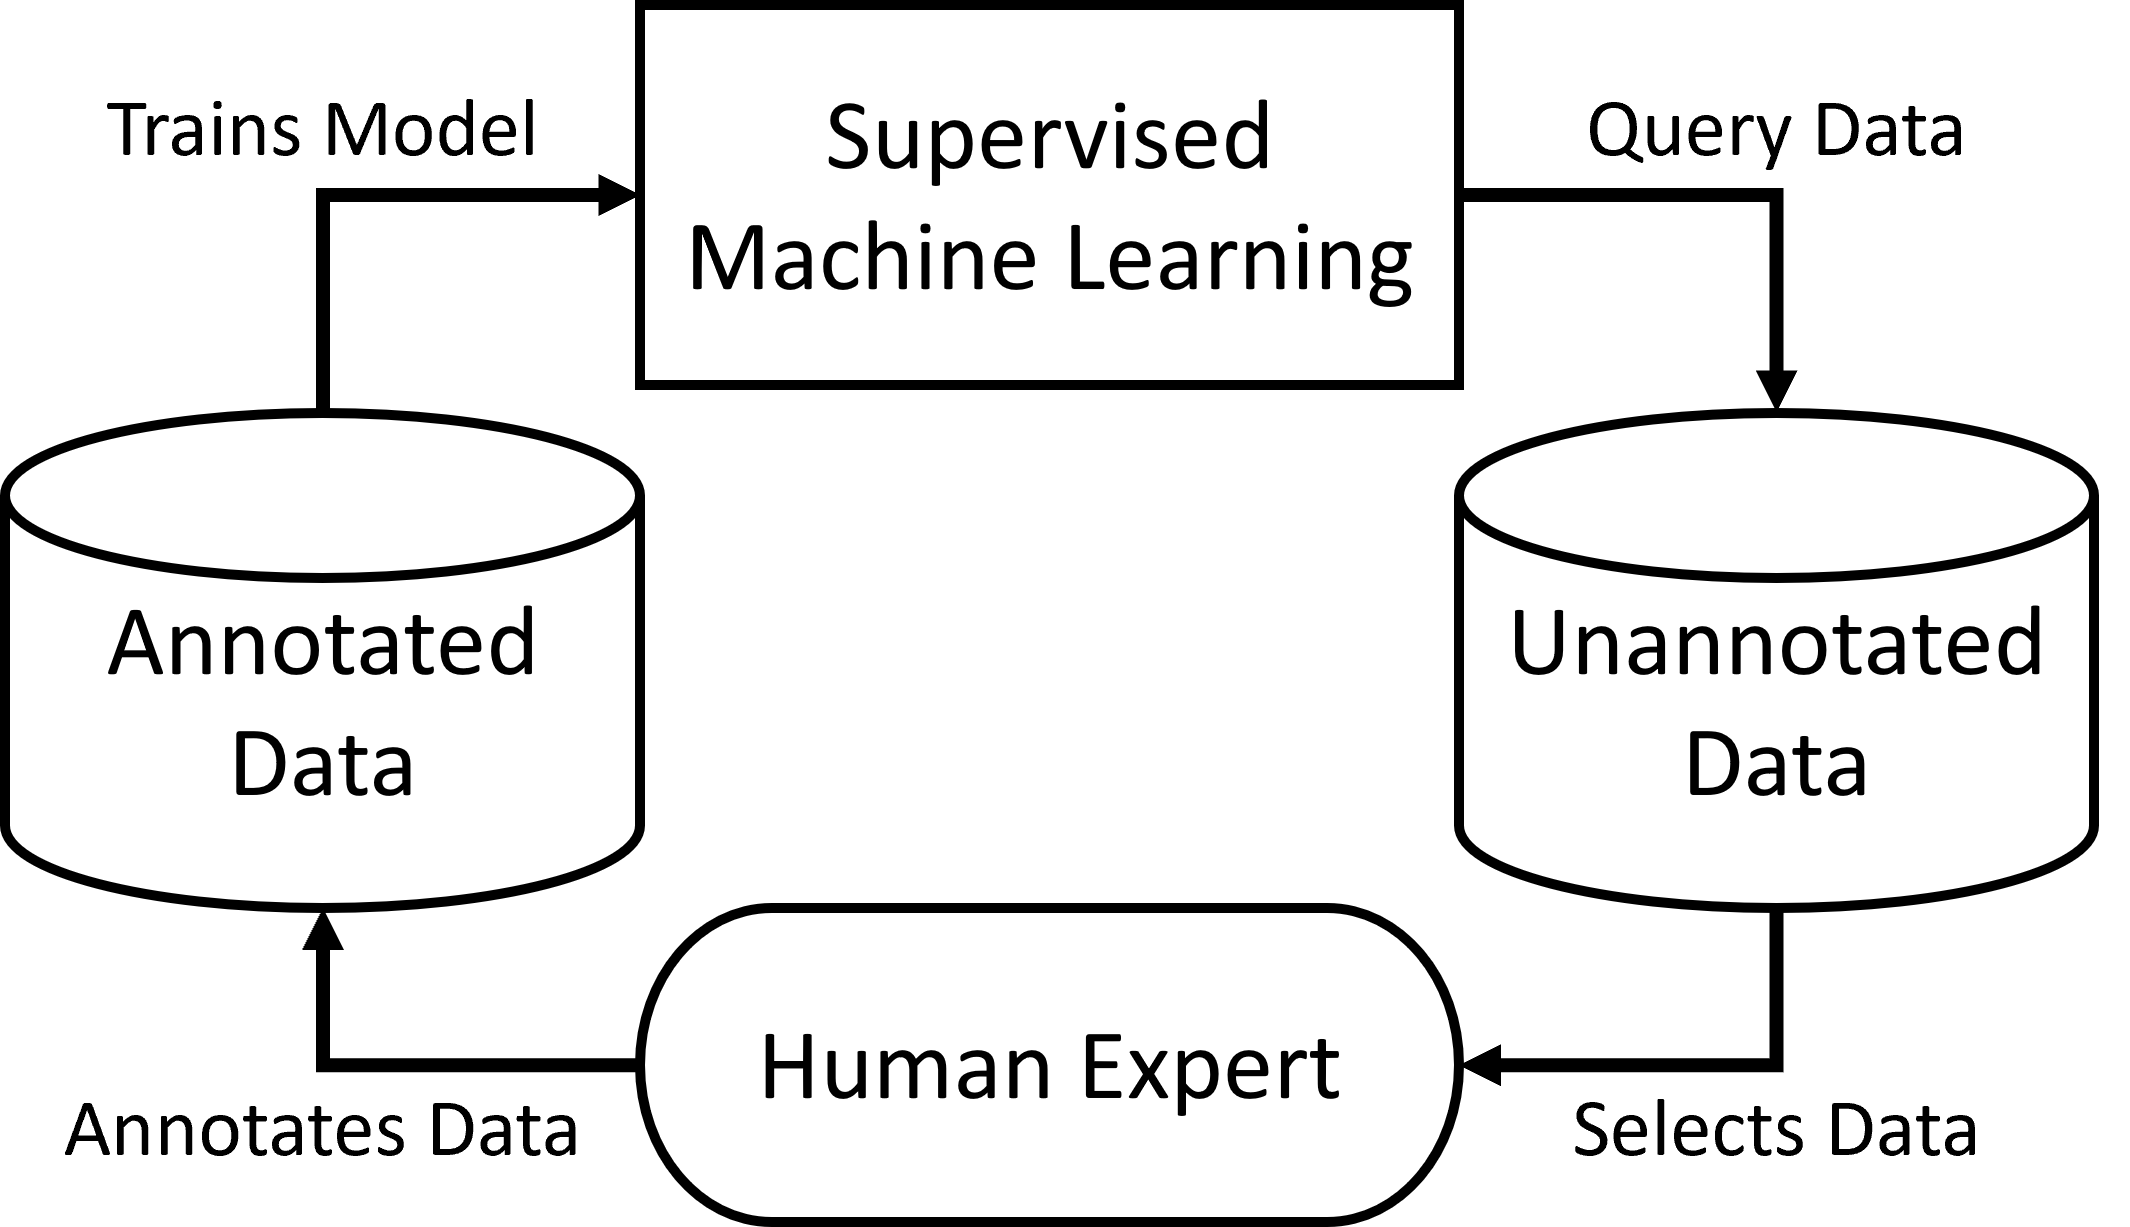
\includegraphics[width=0.75\textwidth]{images/active_learning.png}
	\caption{Pool-based active learning framework.}
	\label{fig:pool_based_active_learning}
\end{figure}

For instance, in the field of dermatology, active learning can be employed to identify representative samples from a vast pool of unannotated images, which can then be annotated by dermatologists. By adopting this strategy, the dermatologist can concentrate on the most informative images, instead of annotating images at random, despite limitations in the amount of annotated data that can be generated, which is often due to financial or temporal constraints. Consequently, by selectively annotating the most informative images, active learning has the potential to enhance the performance of the resulting machine learning model, thereby reducing the need for additional annotated examples.

Active learning has demonstrated its efficacy in traditional machine learning environments, but its applicability in conjunction with deep learning algorithms is subject to limitations that can potentially impede its effectiveness. A particular issue that arises is a selection bias problem~\citep{sener2017active}, as active learning algorithms tend to prioritise the selection of the most informative samples. This can engender a biased dataset that is not reflective of the entire population, ultimately resulting in a deep learning model that acquires feature representations that are not generalisable to unseen data. Consequently, suboptimal classification performance can occur.

Active learning has been shown to be effective in mitigating issues arising from the limited annotation budget; however, further improvements in performance can be achieved by maximising the utility of the unannotated pool. One approach to achieving this is through unsupervised representation learning, which is capable of learning representative features from unannotated images~\citep{bengio2013representation}. The acquired representation can then be transferred to other models, thereby reducing the amount of annotated data required to produce a high-performing model. This can help to alleviate the burden on the active learning algorithm in balancing the selection of representative and informative samples. Unsupervised representation learning is typically achieved using either generative or self-supervised methods.

A generative method aims to learn by generating new examples, such as an autoencoder model that compresses its input data into a lower-dimensional latent space and then reconstructs the original data. The learned latent space can be reused as an encoder in a classification model, which can then be trained in a supervised fashion. In contrast, a self-supervised representation method creates a task for itself, which can be trained in a supervised fashion. One example of this is the RotNet method~\citep{gidaris2018unsupervised}, which involves rotating images and having the model predict the rotation of the image. This approach allows the model to be trained using standard supervised practices, and the learned representations can subsequently be transferred to other tasks. By leveraging these unsupervised representation learning methods, it is possible to extract meaningful features from unannotated data, thereby reducing the burden of annotation and improving the performance of downstream machine learning tasks.

\section{Triage Misdiagnosis}
The limited annotation and the utilisation of techniques to enhance the performance of a specified task may compromise the model's robustness towards images that are outside its training data, such as new disease classifications or diverse image capture conditions. Consequently, the model must be trained to acknowledge the certainty of its predictions, which presents a challenge for deep learning algorithms due to their lack of interpretability and inadequately calibrated predictive probabilities. Therefore, it is imperative to investigate methods to better calibrate deep learning algorithms and adopt selective classifications approaches to reject images that the model is ill-equipped to handle.

Calibration denotes the systematic procedure of conforming the anticipated probabilities of a model with the authentic probabilities of the target variable. When applied in the realm of deep learning, this procedure necessitates adapting the model's output to match the actual distribution of outcomes in the population under consideration~\citep{guo2017calibration}. Generally, three distinct methodologies are utilised to improve the calibration of deep learning algorithm outputs, namely model regularisation, post-hoc calibration, and Bayesian neural networks. Model regularisation involves the imposition of regularisation during the training phase, while post-hoc calibration entails fine-tuning the output probabilities after the model has undergone training. Additionally, Bayesian neural networks are acknowledged to be intrinsically superior for calibration purposes.

Selective classification, or classification with a reject option~\citep{chow1957optimum}, represents a machine learning approach that entails the assignment of one of several conceivable labels to an input image or region of interest, while also incorporating an extra option to reject the image or label it as unknown (Figure \ref{fig:selective_classification}). The integration of a reject option in the classification process permits the system to circumvent erroneous diagnoses or recommendations when the input image's classification is uncertain. In lieu of making an incorrect prediction, the system can request supplementary information or refer the image to a human expert for further evaluation. One prevalent strategy for selective classification involves establishing a threshold on the confidence score generated by the classifier, if the confidence score falls below the threshold, the image is discarded.

\begin{figure}[h]
	\centering
	
\includegraphics[width=0.5\textwidth]{images/selective_classification.png}
	\caption{Selective Classification framework.}
	\label{fig:selective_classification}
\end{figure}

The use of asymmetrical costs is a modification that can be implemented to address the varying costs associated with misclassifications stemming from false positives and false negatives. False positives refer to cases where a healthy patient is incorrectly diagnosed as having a disease, while false negatives denote instances where a patient with a disease is erroneously identified as healthy. The consequences of these types of misclassifications can be vastly dissimilar. In the context of a skin lesion classification scenario, a false positive may lead to unnecessary and potentially harmful interventions such as biopsies, additional testing, and heightened anxiety. Conversely, a false negative could result in delayed treatment, missed diagnoses, and ultimately, a worsened patient outcome. The integration of selective classification alongside asymmetrical costs may yield selective classification systems that reject images that could lead to higher costs if misdiagnoses, thereby minimising the costs associated with such misclassifications.



\section{Dataset Generalisation}
The majority of research in the field of medical image analysis employs open-source datasets. Open-source datasets are publicly released datasets intended to facilitate further research. While such datasets have aided advancements in this area, the resulting machine learning models are often not amenable to generalisation across disparate datasets captured at different sites~\citep{chin2022prepare}. It is essential for machine learning models to generalise across medical data from distinct capture sites to achieve broad applicability and effectiveness in diverse clinical contexts. Failure to do so may result in suboptimal performance and inaccuracies that can adversely impact clinical decision-making in medical applications where precision and accuracy are paramount. For example, if a model trained on imaging data from one hospital is applied to imaging data from a different hospital that employs distinct imaging technology, it may generate erroneous results that could lead to incorrect diagnoses and treatments.



\section{Research Questions and Contributions}
\label{sec:research_contributions}
Drawing from the aforementioned motivations, this thesis centres on the following research questions:

\begin{itemize}
	\item \textit{How can a deep learning model be effectively trained to achieve optimal performance when faced with a scarcity of annotations, and a large corpus of unannotated data?}
	\item \textit{To what extent can selective classification techniques be applied in order to mitigate the costs associated with asymmetrical misdiagnosis of skin lesion images?}
\end{itemize}

\noindent To provide solutions to the questions, this thesis presents the subsequent contributions:

\begin{itemize}
	
	\item An active learning framework specifically for histopathology patches, which serves to enhance annotator efficiency and optimize the volume of nuclei annotations (\textbf{Chapter~\ref{ch:active_learning}}).
	
	\item A modified state of the art unsupervised representation learning algorithm, Multi-Directional Contrastive Predictive Coding, specifically tailored for pathology images that lack a discernible directionality (\textbf{Chapter~\ref{ch:unsupervised_representation_learning}}).
	
	\item An empirical investigation of deep learning calibration techniques for both multi-class dermatology and binary histopathology patches. The examination encompasses Bayesian neural networks, model regularisation, and post hoc methods (\textbf{Chapter~\ref{ch:classification_claibration}}).
	
	\item A comparative analysis of selective classification techniques, in both binary and multi-class scenarios that encompasses Bayesian neural networks, calibrated neural networks, and specialized models designed for selective classification (\textbf{Chapter~\ref{ch:selective_classification}}).
	
	\item Study of deep learning algorithms, specifically their capacity to generalize across various dermatology datasets from distinct sources, some of which were referred for dermatologist examination, and larger open-source dermatology datasets (\textbf{Chapter~\ref{ch:dataset_generalisation}}).
	
\end{itemize}

\noindent This thesis does not primarily aim to create original deep learning techniques. Instead, it strives to devise innovative approaches by amalgamating existing methods to tackle challenging inspection applications.



\section{Thesis Structure}
\label{sec:thesis_structure}
The thesis has been methodically organized into separate chapters corresponding to the major contributions made. Each chapter encompasses an exposition of the underlying motivations, a survey of the pertinent literature, and an account of the conducted experiments. Herein, we present a succinct overview of the individual chapters:

\subsection*{Annotator Efficient Active Learning}
With the increasing popularity of deep learning in medical image analysis and digital pathology~\citep{tizhoosh2018artificial}, it has become increasingly crucial to develop methods that can reduce the need for costly data annotations. Active learning is a promising approach to minimize the amount of annotated data required to train machine learning models~\citep{settles2012active}. However, the effectiveness of traditional active learning strategies with deep learning is limited~\citep{wang2016cost}. In patch-based machine learning systems, active learning methods typically request annotations for individual small patches, which can be laborious and expensive for annotators who must rely on visual context. To address this issue, we propose an active learning framework that selects regions for annotation that are composed of multiple patches, which is expected to increase annotation throughput~\citep{carse2019active}. We evaluated the framework with various query strategies on the task of nuclei classification, using convolutional neural networks trained on small patches containing single nuclei. Traditional query strategies performed worse than random sampling.

\subsection*{Unsupervised Representation Learning}
Recent advancements in deep learning algorithms have had a significant impact on digital pathology tasks. However, a significant challenge in this field is the need for large amounts of annotated data. To overcome this issue, unsupervised learning techniques, particularly contrastive predictive coding (CPC)~\citep{oord2018representation}, have been proposed to leverage abundant but unannotated data for training classifiers. In this chapter, a modification to the CPC framework for use in digital pathology patch classification is purposed, which involves the use of an alternative mask to construct the latent context and a multi-directional PixelCNN autoregressor~\citep{oord2016pixel}. Using the Path Camelyon histology patch dataset~\citep{veeling2018rotation}, it is demonstrated that this purposed method can produce effective deep feature representations for improved classification accuracy in digital pathology when compared to the standard implementation of CPC~\citep{carse2021unsupervised}.

\subsection*{Predictive Probability Calibration}
It is well established that deploying deep learning classifiers for medical image analysis tasks requires careful consideration of issues related to predictive calibration~\citep{maron2019systematic}. Mis-calibration, defined as the discrepancy between predictive probability (confidence) and classification correctness~\citep{guo2017calibration}, can significantly impact the ability to make cost-sensitive and selective decisions~\citep{carse2021robust}. To understand the effectiveness of various calibration methods, an empirical study was conducted on two medical image datasets: one for multi-class dermatology classification and one for binary histopathology image classification. The study applied the temperature scaling method, in which the temperature parameter is optimized using various calibration measures instead of the standard negative log-likelihood, to networks trained with one-hot encoding and cross-entropy loss, as well as networks trained with focal loss and label smoothing. The results of these methods were compared to those obtained using two Bayesian neural network approaches. The findings suggest that while alternative calibration metrics may not offer significant advantages for tuning temperature, temperature scaling of networks trained with focal loss and appropriate hyperparameters demonstrated strong performance in terms of both calibration and accuracy across both datasets~\citep{carse2022calibration}.

\subsection*{Asymmetrical Selective Classification}
Skin lesion classifiers must enable decision-making that is sensitive to cost. This chapter investigates techniques for selective, cost-sensitive classification in both binary triage and multi-class disease classification scenarios, using misclassification costs provided by clinical dermatologists based on healthcare economics. The chapter evaluates various methods of uncertainty estimation with neural networks and probability calibration. Additionally, a modification to SelectiveNet~\citep{selective2019geifman}, called EC-SelectiveNet~\citep{carse2021robust} is purposed, that discards the selection head during testing and relies on expected costs to make decisions. The results demonstrate the advantages of training for full coverage, even when operating at lower coverage, and show that EC-SelectiveNet outperforms standard convolutional neural networks using temperature scaling~\citep{guo2017calibration} or Bayesian neural networks using different measures of uncertainty, in both symmetric and asymmetric cost settings.

\subsection*{Cross Site Generalisation}
This chapter examines the generalisability of deep neural network classifiers for macroscopic skin lesion images in the NHS of the UK. Although deep learning has shown promise in dermatology, its ability to accurately diagnose macroscopic skin disease images that lack dermoscopic information remains a significant challenge~\citep{jones2022artificial}. To address this, four diagnostic image datasets were utilised, including two locally-sourced datasets and two publicly available datasets. Two types of neural network models were trained and evaluated on each dataset, with pre-training on the SD-260~\citep{yang2019self} dataset followed by fine-tuning on the target domain data showing the most promising results. This study emphasises the importance of assessing the generalisability of deep learning algorithms for macroscopic skin lesion images in real-world settings and highlights the potential benefits of utilising vast public macroscopic datasets for pre-training and fine-tuning. Future research is necessary to evaluate the generalisability of these algorithms across different populations and acquisition settings.

\subsection*{Conclusion}
This chapter presents a thorough and exhaustive examination of the research conducted, elucidating its contributions and limitations while highlighting the potential for cost-effective annotation and predictive triage diagnosis in the realm of medical image analysis, with particular emphasis on histopathology and dermatology. Moreover, this chapter lays the groundwork for future research to build upon these findings. This chapter underscores the criticality of mitigating annotation costs and triage misdiagnosis to promote the widespread utilization of medical image analysis systems in clinical settings.